\documentclass[a4paper,12pt,twoside]{article}
\usepackage[inner=3cm,outer=2.5cm,top=2.5cm, bottom=2.5cm]{geometry} %left=4cm,right=2cm would be equivalent
\usepackage[utf8]{inputenc}
\usepackage{t1enc}
\usepackage{graphicx}
\usepackage[magyar]{babel}
\usepackage[nottoc]{tocbibind}%hogy az irodalomjegyzék is benne legyen a tartalomjegyzékben
\usepackage{pdfpages}

\usepackage{commath} %abszolút érték jelhez.
\usepackage{multirow}
\usepackage{subcaption}
\usepackage{subfig}
%matgót megoldottam a 2. sorban.
%\usepackage{anysize} %margóhoz
%\marginsize{3cm}{3cm}{2.5cm}{2.5cm}


%ha esetleg ki akarod szerni az összes ábrát ->
%\usepackage{comment}
%\excludecomment{textcolor}
%\excludecomment{figure}
%\let\endfigure\relax
%<-
\linespread{1.3} %1.3 = másfélszeres sorköz.
%\usepackage{showframe} -> megjelnnek a margók.

\begin{document}
\frenchspacing
%%%%%%%%%%%%%%%%%%%%%%%%%%%%%%%%%%%%%%%%%%%%%%%%%%%%%%%%%%%%%%%%%


\pagenumbering{gobble}

 \begin{center} \includegraphics[width=80mm,keepaspectratio]{abrak/bmelogo.jpg}\\ \vspace{0.3cm}  \Large Diplomamunka \\[1.5cm] \vspace{0.5cm} { \large \textbf{ Mikro-CT készülék rekonstrukciós és kalibrációs környezetének létrehozása}}\\[2.5cm] \vspace{0.2cm} \large Marinovszki Árpád\\[5cm] \begin{tabular}{ll} Témavezető: & Dr.\ Légrády Dávid \\ & egyetemi docens \\ & BME Nukleáris technika Intézet \\ \end{tabular} \vfill \large BME \\ \large 2016 \end{center} 
 
 \clearpage \setcounter{page}{1}
 \pagenumbering{arabic}
 
   \includepdf[ pagecommand={}]{abrak/jelentkezes.pdf}

\clearpage

{\large Önállósági nyilatkozat}
\\[0.5cm]



Alulírott Marinovszki Árpád a Budapesti Műszaki és Gazdaságtudományi Egyetem fizikus MSc szakos hallgatója kijelentem, hogy ezt a diplomamunkát meg nem engedett segédeszközök nélkül, önállóan, a témavezető irányításával készítettem, és csak a megadott forrásokat használtam fel. 


Minden olyan részt, melyet szó szerint, vagy azonos értelemben, de átfogalmazva más forrásból vettem, a forrás megadásával jelöltem.
\\[0.3cm]

Budapest, 2016.\ június 6.

\hspace{9cm}\makebox[1.5in]{\hrulefill}

\hspace{9cm}\makebox[1.5in]{\centering aláírás}




\clearpage


 \tableofcontents

\clearpage

	






%CSAPJUNK A LECSÓBA
%TODO majd egyeztesd az egyes fejezeteken belül a személyeket és az igeidőt (csináljuk / csinálják/ csinálták stb)
%BEVEZETÉS------------------------------------------------------
\section{Bevezetés}

\section{Gain korrekció}


A gain korrekció az elkészült felvételeken elsődlegesen elvégzendő korrekció, amely felelős egyrészt azért, hogy a detektorpixelek eltérő érzékenysége és zaja következtében fellépő képhibákat eltüntesse. Továbbá, hogy korrigálja a röntgennyaláb mért intenzitásában történő azon gyengülést, amely pusztán azért következik be, mert a detektorpixelek más--más távolságra vannak a forrástól.

A fejezet elején megmutatom, hogy milyen hibákat eredményez a gain korrekció elhanyagolása. Ez után ismertetem a korrekció elvégzéséhez szükséges algoritmusokat, majd bemutatom, hogy implementáltam ezeket az elkészült programban. 

\subsection{A gain korrekció által javított artefaktumok bemutatása}

A gain korrekció által kiszűrt hibák három részre oszthatóak. Egyrészt belátható, hogy a sík detektoron mérhető fluxus értéke nem egyenletes. Ha olyan felvételt tekintünk, ahol nincs leképezendő objektum, belátható, hogy a legnagyobb fluxus a detektor azon pixelét fogja érni, amely a legközelebb van a röntgenforrás fókuszpontjához. Az ettől távolabbi pixeleken mérhető intenzitás pusztán azért is kisebb lesz, mert a forrásponttól távolabb vannak, hiszen a mérhető intenzitás a fókuszponttól számított távolság négyzetének inverzével arányos. A jelenség következtében tehát a detektorpixelek intenzitása a szélek felé csökken, és a csökkenés mértéke az expozíciós beállításoktól -- úgy mint az expozíciós idő, valamint a röntgencső feszültsége és árama -- független. A kialakult képtorzulást \emph{flatness hibának} nevezzük, utalva arra, hogy ez azért következik be, mert a detektorunk sík -- gömbfelületű detektornál ez a hiba nem lépne fel.

Megállapítható továbbá, hogy a detektorpixelek eltérő érzékenysége miatt is fellépnek képhibák. Ezen hibákat két csoportra lehet bontani: \emph{offset hibára}, valamint \emph{gain hibára}. Az elnevezés igen szemléletes. Válasszunk ki a detektoron egy adott pixelt, és vizsgáljuk ennek a pixelnek az mért intenzitását, miközben változtatjuk az expozíciós időt! Az adott pixelen a mért intenzitás -- expozíciós idő függvényt ábrázolva olyan görbét kapunk, amely kezdetben igen jó közelítéssel egyenest mutat, mígnem az intenzitás egy adott értéket elérve nem nő tovább. Utóbbi esetet, azaz, amikor az intenzitásérték tovább nem nő, szaturációnak hívjuk. Az előbbihez hasonlóan, ha állandó expozíciós idő mellett a röntgencső áramerősségét változtatjuk, és így nem a felvétel idejét növeljük, hanem a detektorra eső nyalábintenzitást, szintén kezdetben lineáris, majd telítődő összefüggést kapunk a pixel által mért intenzitás -- alkalmazott áramerősség függvény tekintetében. Éppen ezért az expozíciós idő és a röntgencső áramerősségének szorzatának -- a továbbiakban \emph{expozíció} függvényében szokás vizsgálni az adott pixel intenzitását. Az így kapott görbe, azaz az intenzitás az expozíció függvényében, adja meg az adott pixel érzékenységét.

Ez az érzékenység azonban pixelről pixelre változik. Különböző pixelek érzékenységét megvizsgálva észrevehetjük, hogy az egyes érzékenységi görbék lineáris szakaszának meredeksége és tengelymetszete is változik. Változik továbbá a szaturációs expozíció is, azaz az az expozíció érték, amelynél az adott detektor telítésbe megy. Ezt szemlélteti \aref{fig:gaingrafikon}.~ábra, amelyen négy különböző pixel által mért intenzitást ábrázoltam, az expozíció függvényében. Az ábrán jól látszódik, hogy a különböző pixelek érzékenysége eltérő meredekségű és tengelymetszetű egyenessel jellemezhető, valamint a szaturációs expozíciójuk is eltérő. Az offset és gain korrekciók a detektorpixelek ezen érzékenységbeli különbségeit korrigálják. Az \emph{offset hibák} javítása jelenti a lineáris szakaszok eltérő tengelymetszetőből származó eltérések kiküszöbölését. Az offset  hibák nagysága nem függ tehát az expozíciótól, de függ az expozíciós időtől. Ugyanis kikapcsolt röntgenforrás mellett is detektálunk valamekkora háttérsugárzást, illetve a detektorok zaja is mérhető intenzitást fog eredményezni a felvételen. A teljes, röntgenforrás nélkül mért jel tehát arányos lesz az expozíciós idővel és függeni fog a pixelek érzékenységétől is.  A \emph{gain hibák} javítása jelenti az érzékenységek lineáris szakaszainak eltérő meredekségéből, valamint az eltérő szaturációs expozíciókból származó hibák javítását. Ezek tehát az expozíciós beállításoktól függő hibák.





\begin{figure}[htbp]
\center
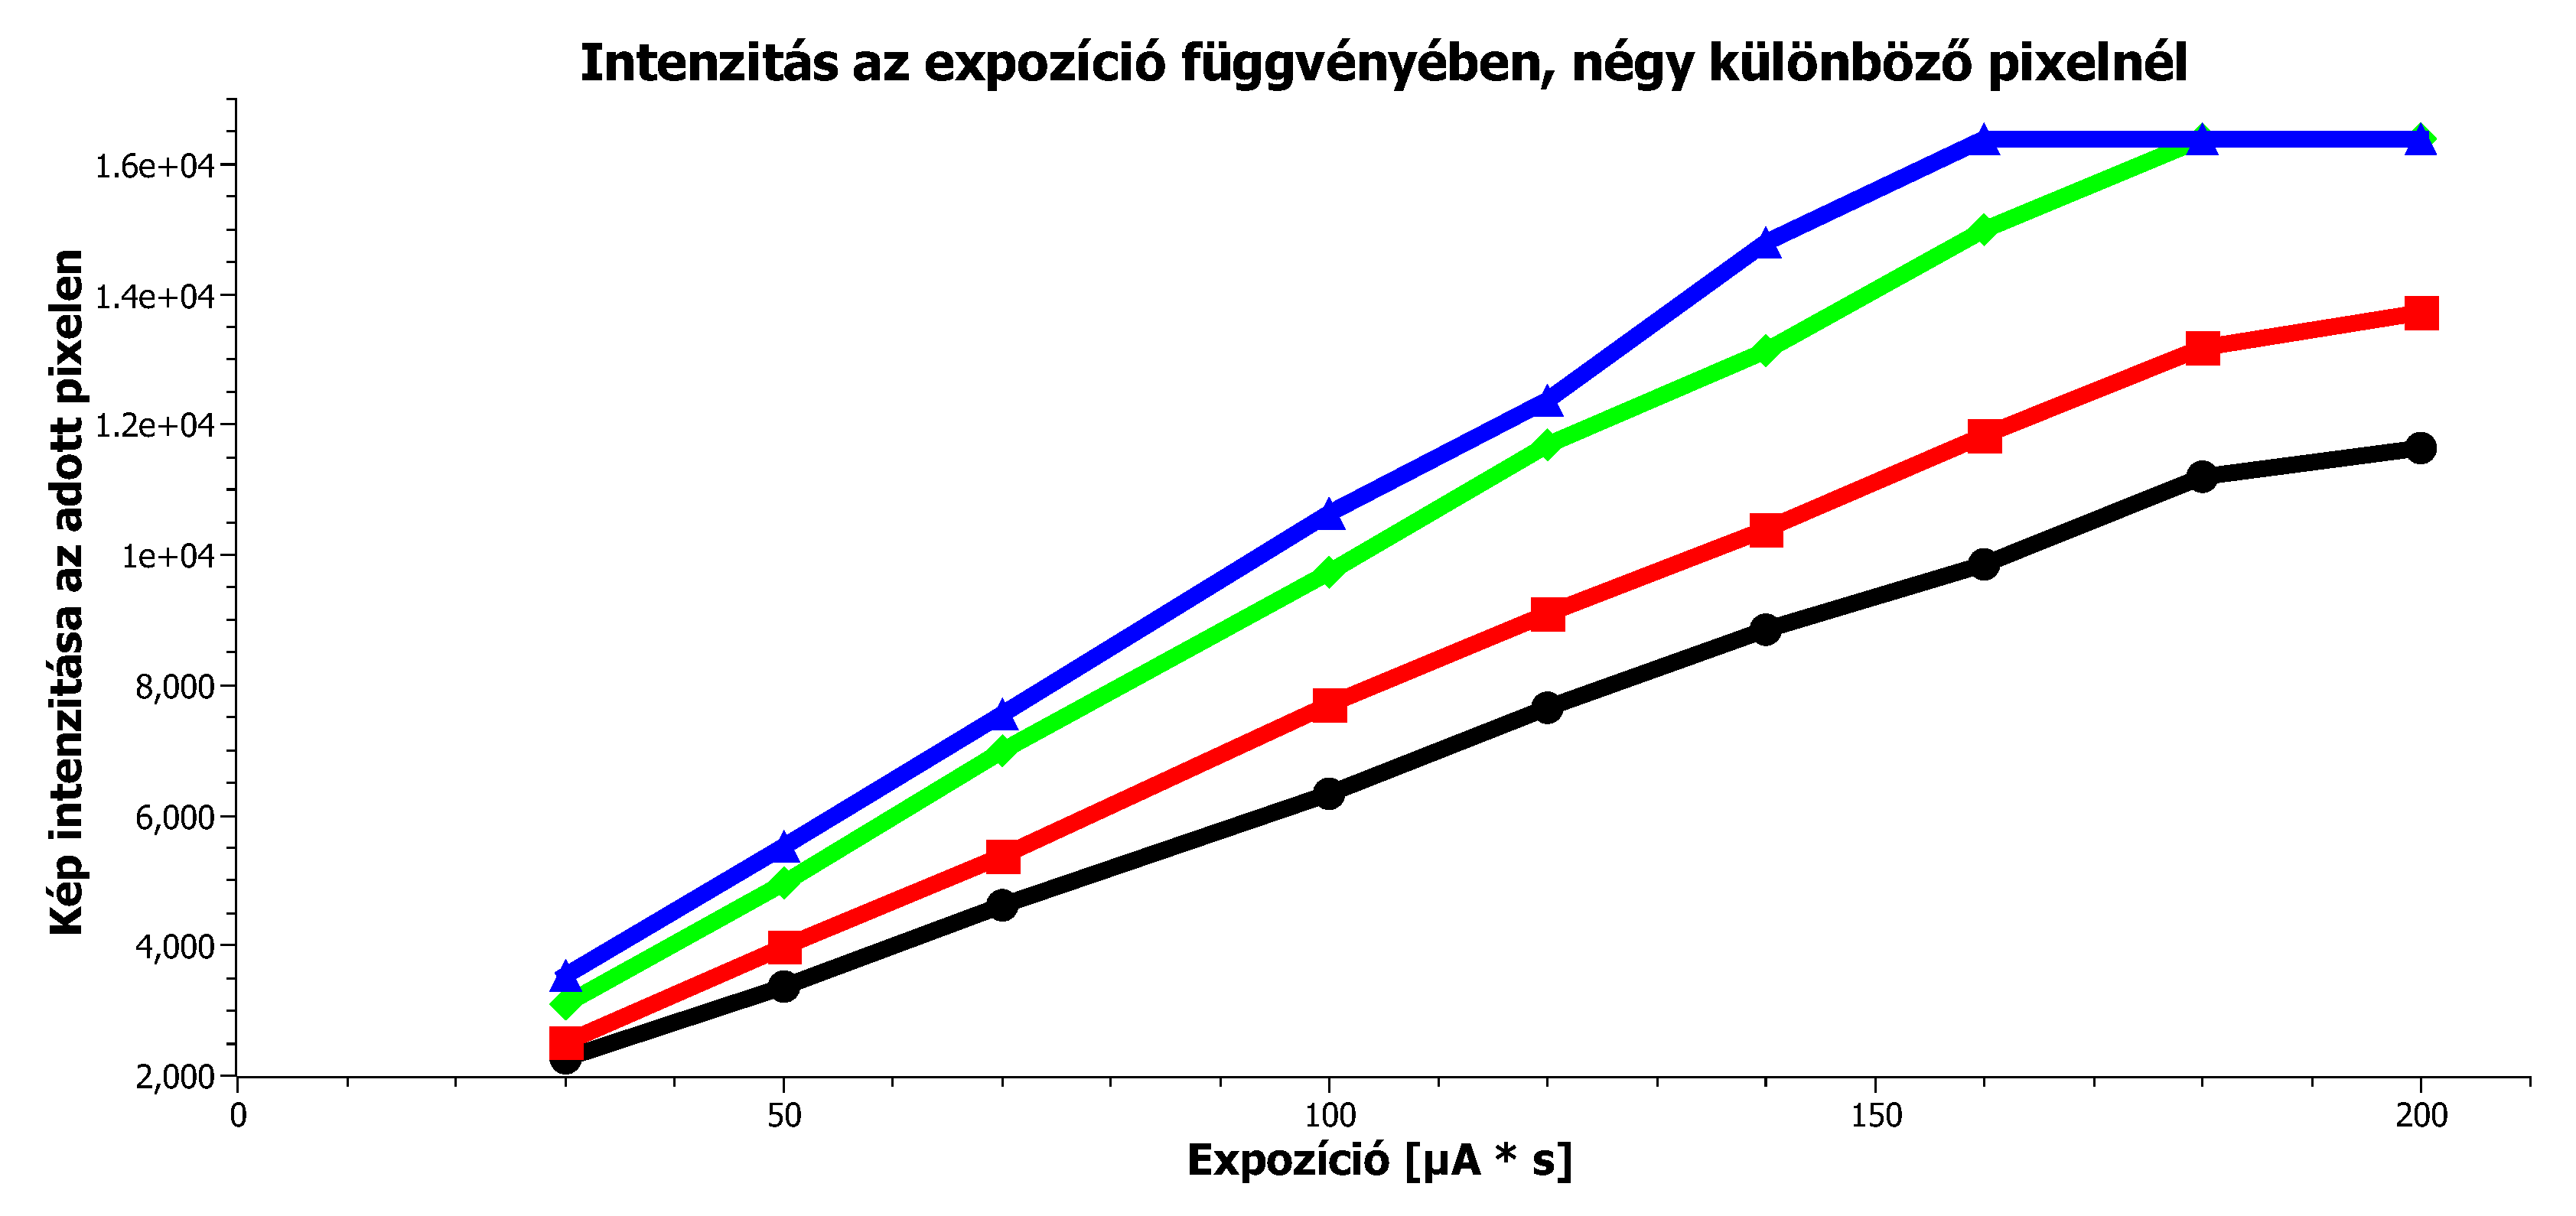
\includegraphics[width=0.8\textwidth]{abrak/gaingrafikon}
\caption{Négy kiszemelt pixel intenzitásának változása az expozíció függvényében.}
\label{fig:gaingrafikon}
\end{figure}




Az egyes hibák hatását az elkészült felvételeken \aref{fig:gainnelkul}.~ábrán szemléltetem. Az ábrán egy olyan felvétel látható, amely készítésekor a detektor és a forrás között leképezendő objektum nem volt, továbbá a felvétel mindenféle korrekciótól mentes, azaz a mérőszoftver ezt a képet olvasta ki a detektorból. Az ábrán látható, hogy a leképezendő objektum hiányában homogénnek várt kép közel sem homogén. Általánosan megfigyelhető, hogy az egyes pixelek értékei jócskán szórnak, továbbá látható, hogy a képen négyzetrácsos struktúra rajzolódik ki, amelynek oka valószínűleg az detektorpanelek határainál megváltozik a pixelek érzékenysége. Különösen határozott ez az eltérés a képen látható hat függőleges egyenes mentén. Ezen pixelek az összes felvételen alacsonyabb intenzitással rendelkeznek társaiknál és értékük is kevésbé változik az expozíció növelésével, mint a többi pixel. Megfigyelhető továbbá, hogy a kép egyre sötétebb a sarkok felé, amely a flatness hibáak tudható be.

\begin{figure}[htbp]
\center
\includegraphics[width=1.0\textwidth]{abrak/gainnelkul}
\caption{Tárgy nélkül készített felvétel, gain korrigálás nélkül.}
\label{fig:gainnelkul}
\end{figure}

A gain korrekció során tehát ezen hibákat távolítjuk el a képről. Gain korrekció után a fenti képből \aref{fig:gainnel}.~ábrán látható képet kapjuk. Megfigyelhetjük, hogy itt nem látszódnak az előbb jelölt artefaktumok. Bár a kép továbbra sem teljesen homogén -- ezt nem is várjuk el, valamekkora zaj mindenképp terhelni fogja a méréseinket --, a pixelek intenzitásának szórása jóval lecsökkent, megszűnt a gain korrekció nélküli képet átható négyzetes struktúra, és a kevésbé érzékeny pixelek sem lógnak ki a többi közül. A következőkben a gain korrekcióhoz szükséges algoritmusokat ismertetem.

\begin{figure}[htbp]
\center
\includegraphics[width=1.0\textwidth]{abrak/gainnel}
\caption{Tárgy nélkül készített felvétel, gain korrigálás után.}
\label{fig:gainnel}
\end{figure}

\subsection{A gain korrekció algoritmusai}

A felvételek gain korrigálásához először is meg kell határozni az egyes detektorpixelekhez tartozó érzékenységeket, azaz azt, hogy az expozíció növelésével milyen gyorsan változik a pixel intenzitása, valamint azt, hogy az adott pixel milyen expozíció melett telítődik. ezen kívül meg kell határozni, hogy megvilágítás nélkül hogyan változik az adott pixel intenzitása az expozíciós idő függvényében. Ehhez először kalibráló képsorokat kell készíteni. Az offset hibák javításához a röntgenforrás bekapcsolása nélkül, különböző expozíciós időkkel, a gain és flatness hibák javításához bekapcsolt forrással, különböző expozíció értékek mellett. 

A képeket először az offset hibáktól kell megszabadítani. Az ehhez szükséges korrekciós faktorok meghatározásához tehát különböző expozíciós időkkel, kikapcsolt forrással készítünk képeket. Az egyes pixelek értékét az expozíció idő függvényében ábrázolva olyan görbét kapunk, amelyre jól illeszthető egyenes. Ez alapján az $i$. pixel által, forrás nélkül mért $ I_i^{\text{offset}}$ intenzitás \aref({eq:offset}) képlettel írható le, ahol $a_i^{\text{offset}} $ és $b_i^{\text{offset}}$ a fenti módon előállított képsorozatból, egyenes illesztéssel megkapható és pixelenként változó.

\begin{equation}
\label{eq:offset}
I_i^{\text{offset}} =  a_i^{\text{offset}} \cdot t_{\text{exp}} + b_i^{\text{offset}}
\end{equation}

Minthogy ezek az intenzitásértékek a detektort érő hasznos jeltől függetlenül megjelennek, először ezen értékeket kell levonni az elkészült képekből. 

Az offset hibák korrigálása után tehát az $i$. pixel intenzitása \aref({eq:offsetkorr})~ képlet szerint alakul, ahol $I_i^{\text{mért}}$ az $i.$ pixel eredeti, korrekció nélküli intenzitása, $I_i^{\text{offsetkorrigált}}$ pedig az offset hibától mentes érték.

\begin{equation}
\label{eq:offsetkorr}
\begin{split}
I_i^{\text{offsetkorrigált}}  &=  I_i^{\text{mért}} - I_i^{\text{offset}} \\&=  I_i^{\text{mért}} - \left( a_i^{\text{offset}} \cdot t_{\text{exp}} + b_i^{\text{offset}} \right)
\end{split}
\end{equation}


Ez után javíthatjuk ki a gain és flatness hibákat. A két hiba valójában egy algoritmussal javítható, hiszen a flatness hiba felfogható úgy, mintha a detektor pixeleinek érzékenysége lenne más a detektor más--más területein. A szükséges korrekciós faktorok meghatározásához olyan kalibráló képsorokat kell készítenünk, amelyek különböző expozícióval készülnek. \Aref{fig:gaingrafikon}.~ábrán látottak alapján megállapítható, hogy az egyes detektorpixelek intenzitása kezdetben az expozícióval lineárisan változik, vagyis egyenest tudunk rá illeszteni. Amennyiben tehát nincs tárgy a detektor és a forrás között, az $i$. pixel által, a detektort érő sugárzás, mint hasznos jel által okozott ( tehát offset hibától mentes) $ I_i^{\text{offsetkorrigált}}$  intenzitás értéke \aref({eq:gain})~egyenlet szerint számolható az expozícióból. Itt $a_i^{\text{gain}}  $ és $b_i^{\text{gain}}$ jelöli a különböző expozíciós értékek mentén felvett intenzitásértékekre illesztett egyenes paramétereit, $E$ pedig az expozíció értékét, amely a fent leírtak alapján az expozíciós idő és a röntgencső áramának szorzata.

\begin{equation}
\label{eq:gain}
\begin{split}
I_i^{\text{offsetkorrigált}}  &=  I_i^{\text{mért}} - I_i^{\text{offset}} \\&=  a_i^{\text{gain}} \cdot E + b_i^{\text{gain}}
\end{split}
\end{equation}

Egy olyan felvételen, amely készítésekor valamilyen tárgyat helyezünk a detektor és a forrás közé, a mért intenzitásértékek nyilván el fognak térni a detektor különböző részein, ahogy a leképezni kívánt tárgy lineáris gyengítési együtthatója is eltér a különböző térfogatokban. Ezt úgy vehetjük figyelembe, hogy  \aref({eq:gain})~képletben az $E$ expozíció érték helyére egy helyfüggő, $E_i^{\text{virt}}$ virtuális expozíciót vezetünk be. Ezen érték úgy módosul az eredeti $E$ expozícióhoz képest, hogy figyelembe veszi a röntgen nyaláb gyengülését, miközben az áthalad a leképezni kívánt tárgyon. Vagyis egy adott mérés során az $E_i^{\text{virt}}$ virtuális expozíció nem lesz más, mint az a (valós) expozíció érték, amely esetén ugyan akkor intenzitást mértünk volna tárgy nélküli elrendezésben, mint jelen esetben a leképezendő tárggyal. Ezzel a jelöléssel kapjuk \aref({eq:gain_virtual}) egyenletet, amely immáron általánosan igaz, egy tetszőleges felvételre -- míg \aref({eq:gain})~egyenlet csak arra az esetre érvényes, amikor nincs semmi a detektor és a forrás között.

\begin{equation}
\label{eq:gain_virtual}
\begin{split}
I_i^{\text{offsetkorrigált}}  &=  I_i^{\text{mért}} - I_i^{\text{offset}} \\&=  a_i^{\text{gain}} \cdot E_i^{\text{virt}} + b_i^{\text{gain}}
\end{split}
\end{equation}


A gain hibák javítása során azt szeretnénk elérni, hogy az egyes pixelek intenzitása ne függjön az adott pixel érzékenységétől, azaz az $a_i^{\text{gain}}  $ és $b_i^{\text{gain}}$  együtthatóktól, csak az adott pixelt ért -- virtuális -- expozíciótól. Vagyis azt, hogy ha két detektorpixelt egy felvétel során ugyanolyan intenzitású sugárzás ér, és az expozíciós idő is megegyezik, akkor a két pixel intenzitása az elkészült képen is azonos legyen. 
Ezt úgy végezzük el, hogy először meghatározzuk az egyes detektorpixelek virtuális expozícióját, majd ezekből úgy alakítjuk ki a gain korrigált intenzitásértéket, mintha minden pixel érzékenysége megegyezne.

Először tehát kiszámoljuk az adott offset korrigált intenzitáshoz tartozó virtuális expozíció értékét \aref({eq:gain_virtual})~egyenlet segítségével. Egyszerű átrendezéssel kapjuk a virtuális expozícióra  \aref({eq:virtual_expozicio})~egyenletet. 

\begin{equation}
\label{eq:virtual_expozicio}
\begin{split}
 E_i^{\text{virt}} &= \frac{I_i^{\text{offsetkorrigált}} -  b_i^{\text{gain}}}{  a_i^{\text{gain}}}
 \end{split}
\end{equation}



 A virtuális expozíció tehát azzal van összefüggésben, hogy mekkora valós fluxus érte az adott pixelt, és mentes az adott pixel érzékenységek torzító hatásától. Ebből úgy határozzuk meg a gain korrigált intenzitás értéket, mintha minden pixel érzékenysége, azaz intenzitás -- virtuális expozíció függvénye egy origón átmenő egyenes lenne, mindnek azonos meredekséggel. A szóban forgó meredekséget pedig úgy határozzuk meg, hogy éppen annál az expozíciós értéknél telítődjön, amelynél a legérzékenyebb pixel már telítődik. Azaz meg kell vizsgálni, hogy az expozíciót növelve mikor kapunk olyan képet, amin már van szaturált pixel. Ezen expozíciót hívjuk szaturációs expozíciónak ($E^\text{szat}$). Ezen érték a kalibráló adatsorból szintén meghatározható paraméter. Ezen paraméter ismeretében a gain korrigált $ I_i^{\text{gainkorrigalt}}$ pixelintenzitás \aref({eq:gainkorrigalt})~egyenlettel számolható, ahol $\left(2^{14} -1\right)$ a detektor maximális intenzitásértéke.

\begin{equation}
\label{eq:gainkorrigalt}
\begin{split}
 I_i^{\text{gainkorrigalt}} &= E_i^{\text{virt}}  \cdot \frac{2^{14} -1}{E^\text{szat}}
 \end{split}
\end{equation}


A módszer hatékonyságát a kísérleti algoritmus létrehozása során Botond részletes tesztekkel vizsgálta, ezért én ettől eltekintek. A továbbiakban azt mutatom be, hogy ezeket az algoritmusokat hogyan építettem bele az elkészült szoftverbe, illetve milyen mérési utasítást ajánlok a korrekciók elkészítéséhez.


\subsection{A gain kalibráció implementálása }


Mint ahogy már említettem  %TODO : említd is, a beveztésben
 a kalibrációs szoftver létrehozásakor szempont volt, hogy annak sebessége gyors, kezelése egyszerű legyen, így létrehoztam egy grafikus felülettel rendelkező programot, amelyben a felhasználó nyomógombokkal tud választani az elérhető funkciók között. Az első ilyen megvalósított funkció az offset és gain hibák korrigálására szolgáló együtthatók meghatározása. Ezt a funkciót választva a szoftver egy új ablakban kéri a felhasználót, hogy  válassza ki az elkészített kalibrációs mérések mappáját, valamint azt a mappát, ahova a kimeneti fájlokat menteni szeretné. Ez után a korrekciós faktorok számolása automatikusan megtörténik, illetve az esetleges hibákról a felhasználó értesítést kap a konzolon.
 
 
A bemeneti fájlok elkészítéséhez, azaz a mérési utasításhoz szükséges megjegyeznem, hogy a mérések során észrevehető volt, hogy a detektor által készített képek egy része valamiért jóval sötétebb, mint az azonos körülmények között készült egyéb képek. Ez a hiba a képek kb.\ 5\%-át érinti, és okát nem sikerült felderíteni. Más felhasználók is panaszkodtak hasonló hibára ennél a detektortípusnál. A korrekciós faktorok számításánál azonban kimondottan fontos, hogy ilyen képeket ne használjunk fel a számításokhoz -- továbbá az ilyen képek kezelése egyéb helyzetekben is szükségszerűnek tűnik. Ennek érdekében a gain kalibrációhoz szükséges méréseket úgy végeztük el, hogy egy adott beállítással több képet készítettünk ( 10--20 képet beállításonként). Az azonos beállításokkal készült képeket külön mappákba mentettük, így a szoftver is ilyen formában várja. Ez a megoldás azért szerencsés, mert egy mappán belül átlagolva a képek intenzitásértékét, könnyen és egyértelműen kiszűrhető, ha valamelyik kép jóval sötétebb, a fent említett hiba miatt. Továbbá az azonos mappákban lévő, tehát azonos beállításokkal készült képeket átlagolva a képeket terhelő zaj is csökken. Így amikor a korrekciós faktorokat számolom, mappánként átlagolom azokat a képeket, amelyek átlagos intenzitása nem tér el 10\%-nál jobban a mappában lévő képek átlagos intenzitásának átlagától. Az program  robusztusságát  tovább növelve, a képek beolvasásakor vizsgálom, hogy  azok milyen expozíciós beállításokkal készültek, és ez alapján is szelektálom a képeket, kiszűrve a mérés során elkövetett emberi hibákat. A mérésvezérlő szoftverről ugyanis tudni érdemes, hogy a felvételek készítésének elindítása a röntgen forrás bekapcsolásától függetlenül elindítható, és az indítás után sorozatosan készít képeket, amíg le nem állítják. Mérés közben a forrás feszültsége és áramerőssége szabadon változtatható, illetve a forrás ki- és bekapcsolható. A röntgencső független kezelése részben biztonságvédelmi célokat szolgál, azonban lehetőséget ad a felhasználónak, hogy a képek sorozatos kimentését elindítsa úgy, hogy a forrás nincs bekapcsolva, vagy a beállított paraméterei nem megfelelők. Ekkor gyakran előfordul, hogy a felhasználó a paramétereket menet közben állítja, és az addigi eredményeket nem törli ki. Ezt kiküszöbölendő, a gain korrekcióhoz készített kalibrációs képek feldolgozása során a képek átlagos intenzitásán kívül a program vizsgálja az átlagos áramerősség, feszültség és exponálási idő paramétereket is, és a kilógó értékkel készült képeket figyelmen kívül hagyja. Továbbá figyelembe veszi azt is, hogy offset korrekcióhoz készült kalibráló képek között ne legyen olyan, ahol a forrás be volt kapcsolva -- vagy ha van, akkor hagyja azt is figyelmen kívül. Hasonlóan a gain és flattness hibák korrigálásához készült képeknél ignorálja az algoritmus azokat a képeket, ahol a forrás ki volt kapcsolva. Amennyiben egy mappában kevés kép van, amely a fenti szűröknek megfelel ( 5nél nem több), akkor a mappa tartalmát a szoftver nem használja fel a korrekciós faktorok meghatározásához. Továbbá, amennyiben túl kevés mappát talál a szoftver, tehát túl kevés a különböző expozíciós beállítások száma a korrekciós faktorok meghatározásához -- akár összesen, akár túl kevés megy át a fenti szűrükön--, a kalibrációs  faktorok nem kerülnek meghatározásra. Így elkerülhető, hogy túl kevés pontra illesszünk egyenest, és ezért hibás eredményeket kapjunk, vagyis a képkészlet ellenőrzése szintén a szoftver robusztusságát növeli. A felvételek elkészítésekor alkalmazott feszültségértékeket az program szintén a képek beolvasásakor határozza meg, így azt külön megadni nem szükséges, mint ahogy a képeket feszültség szerint sem kell szétválogatni -- ellentétben a kísérleti algoritmussal.

A képek beolvasása és mappánkénti  átlagolása után a pixelenkénti egyenes illesztést a szokásos, egyenes illesztésére vonatkozó (\ref{eq:linearfit}) képleteket felhasználva oldottam meg, ahol az $x$ és $y$ mérési pontokra illesztjük az $\alpha$ és $\beta$ paraméterekkel jellemzett egyenest.  A képletben a felülvonás az átlagolást jelenti.

\begin{equation}
\label{eq:linearfit}
\begin{split}
\beta &= \frac{ \overline{xy} - \overline x \cdot \overline y }{\overline{x^2} - {\overline{x}}^2}\\
\alpha &= \overline y -\beta \cdot \overline x
\end{split}
\end{equation}


Jelen esetben $x$ értéke az expozíciós idő (offset hibáknál), vagy az expozíció (gain és flatness hibáknál), y pedig az adott pixel intenzitása. Az egyenes illesztésére egyszerű és gyors megoldásnak találtam, hogy az illeszteni kívánt képeket pixelemként összeadom, valamint ugyanezt megteszem az adott expozícióval -- vagy expozíciós idővel -- megszorozva is, majd ezeket a képeket pixelenként elosztom az összeadott képek számával. Így az $\overline x$ és $\overline{xy}$ értékek pixelenként előállnak, mint egy--egy kép. Ez után a kettő különbségét -- mint képet -- leosztva a $\overline{x^2} - {\overline{x}}^2$ skalárral, közvetlenül előáll a pixelekre illesztett egyenes meredeksége, és a tengelymetszet további képkivonással kapható. Mivel a szükséges képműveletek -- összeadás, skalárral szorzás, kivonás -- könnyen párhuzamosíthatóak, gyakorlatilag az egyenes illesztése is párhuzamosan történik, így jelentősen lerövidítve a számoláshoz szükséges időt. 
%15 perc helyett 2 és fél perc. Az enyém átlagol mappánként, az övé nem.
 A módszer egyébként a memóriával is takarékosabban bánik, mint a kísérleti algoritmus, amely először beolvassa az összes képet a memóriába, majd pixelenként illeszt egyenest. Az ottani megoldással ellentétben, ahol a szükséges memória lineárisan nő a képek számával, nálam a szükséges memória a képek számától független és alacsony.


A fenti megoldáshoz a grafikus felületet és a mappakezelést a Qt biztosítja, míg a gyors képműveletek CUDA kód alkalmazásával valósulnak meg. A képfeldolgozáshoz létrehoztam olyan kép osztályt, amely képes magát fájlból a GPU memóriájába olvasni, és alkalmas a képeken végzett műveletek gyors végrehajtására a grafikus kártyán. A pixelenkénti összeadás, kivonás, skalárral szorzás megoldása viszonylag triviális, itt egy szál egy pixel értékét számolja. Ezzel ellenben a maximum, minimum, átlag, és szórás -- utóbbit a gain korrekcióhoz nem használtam fel, de technikailag itt kell megemlítenem -- számolása első ránézésre nem triviális, ezért néhány mondatban bemutatom. 

Az előbb felsorolt műveletek, amelyek eredménye előáll a kép pixeleiből úgy, hogy minden egyes pixel értékét egyszer használjuk fel, egy kommutatív, asszociatív, két elem között ható -- programozási értelemben vett -- operátorral, az angol irodalom  \emph{reduce} műveletnek hívja. Ilyen az előbb említett összeadás, minimum és maximum számítás is. Például három elem, $a,b$ és $c$ összegét megkapjuk, ha $a$ és $b$ összegéhez hozzáadjuk $c$-t: $\text{sum} = (a+b)+c$. Az összeadást kicserélhetjük maximum számításra is, az algoritmus ekkor csak a számok közé rakott operátorban tér el: $\text{maximum} = \text{max} ( \text{max}(a,b),c))$.  Az ilyen, \emph{reduce} típusú műveletek optimális használatát az összeadás példáján keresztül írom le, de a fentiek értelmében a minimum és a maximum számolás is hasonlóan kivitelezhető.

Az alkalmazásomban is használt reduce műveletet  a CUDA dokumentációjához mellékelt példa\acite{reduce} alapján állítottam össze. Az ilyen műveletek általános megoldása -- az összeadás példáján --, hogy a képet két részre osztjuk, majd az egyik részt hozzáadjuk a másikhoz. A műveletet folytatjuk, mindig felezve a fennmaradó képrészletet, míg végül a kép egyik pixelében előáll az összes pixel összege. A már említett példa ezen túl olyan technikákat is ajánl, mint a \emph{shared memory}, azaz az összes szál által hozzáférhető ( de kívülről nem hozzáférhető), gyors elérésű memória használata -- a lassú elérésű, globális memória helyett, ahol a képek eleve tárolva vannak. Továbbá figyelembe veszi, hogy a párhuzamos futtatás során a szálak 32 darabos ,,csomagokban'',  úgynevezett \emph{warpokban} futnak, ezzel tovább optimalizálva az algoritmust. Míg ha több, mint 32 szálat futtatunk egyszerre, semmi nem garantálja, hogy azok egyszerre fognak futni. Ilyenkor szakaszonként be kell várnia a szálaknak egymást. Például ha a kép egyik felét hozzáadjuk a másikhoz, csak akkor felezhetjük tovább az elkészült képet, ha minden összeadás megtörtént. Amikor már 32-nél kevesebb szálat használunk, akkor a szálaknak nem kell egymást bevárni, hiszen biztosan nem fut több. Továbbá a példa alapján az összeadáshoz vonatkozó kerneleket C++ template-ekkel írtam meg, amely segítségével már fordítási időben tudja a kernel, hogy adott méretű kép esetén hogyan kell felosztani a képet -- nem pedig futási időben kell vizsgálnia, hogy a kép mekkora méretű. 


\subsection{A gain korrekció implementálása}

A korrekciós faktorok meghatározása után, amelyek tehát szintén képként kerülnek mentésre, a felhasználónak lehetősége nyílik az elkészített projekcióit offset és gain korrigálni, az erre vonatkozó (\ref{eq:offsetkorr}) és (\ref{eq:gainkorrigalt}) képleteket felhasználva. Ezek újabb képösszeadásokat és skalárral való szorzást,osztást jelentenek, így az eddig bemutatott függvényekkel gyorsan elvégezhetőek. A felhasználónak ennél a funkciónál is grafikus felületen van lehetősége kijelölni a korrigálni kívánt mappát, amelyből a program az összes képet gain korrigálja és elmenti egy kívánt, kijelölt mappába -- akár ugyan abba. 

%TODO A véletlenszerűen elsötétülő képeket itt is külön korrigálja a program: ha egy kép intenzitása jelentősen eltér a sorrendben mellette lévő képek átlagától, úgy az szoftvera képet a szomszédjainak átlagával helyettesíti a gain korigálás előtt.

\section{A geometria kalibráció}

A diplomaunkám során a másik tárgyalt kalibráció az úgynevezett \emph{geometria kalibráció}, amely a CT-vel elkészített képek alapján állapítja meg, hogy milyen távol van egymástól a detektor, a forgatható asztal forgástengelye és a röntgencső fókuszpontja. A geometriai adatokhoz igen pontosan szükség van, amikor az elkészült projekciók alapján meghatározzuk a felvett tárgy 3 dimenziós képét, vagyis a visszavetítéskor. Ugyanakkor a geometriai paramétereket kézzel nem tudjuk igen pontosan lemérni, már csak azért sem, mert a röntgencső fókuszpontjának a helye nem hozzáférhető és nem ismert, továbbá a mérési pontatlanság is viszonylag nagy lenne. Ezért alkalmazzuk azt a módszert, hogy az elkészült képek alapján határozzuk meg a szóban forgó paramétereket. 



\clearpage

\begin{thebibliography}{9}

\bibitem{reduce}
Mark Harris,
{\it Optimizing Parallel Reduction in CUDA},
{\tt online: http://docs.nvidia.com/cuda/samples/6\_Advanced/reduction/doc/reduction.pdf},
Utolsó hozzáférés: 2016.05.28. 14:00
%(\tt online, }


%\bibitem{url}
%{\tt http://fizipedia.bme.hu/index.php/Gamma\_spektroszkópia},
%2013.~november~29., 1:00

%\bibitem {nagy}
%Nagy L. Gy.,
%{\it Radiokémia és izotóptechnika},
%Tankönyvkiadó, Budapest, 1983.
%\bibitem {lederer}
%C.M. Lederer, J.M. Hollander, I. Perlman,
%{\it \foreignlanguage{english}{Table of Isotopes}},
%Wiley, New York, 1984.
\end{thebibliography}
\end{document}